\chapter{APPENDIX: MC Closure Check}
\label{sec:MCclosureCheck}

To perform the MC closure check, the pseudodata samples are prepared to mimic each of the data samples needed for the fit. This includes:
\begin{itemize}
  \item $W\gamma$-selected samples to be used for fit (full analysis selection without $I_{ch}$ or $\sigma_{i\eta i\eta}$ cuts), those samples are prepared separately for the muon and electron channels;
  \item $W\gamma$ in full selection to be plotted into the [data vs bkg+signal] plots, separately for the two channels;
  \item $Z\gamma\rightarrow\mu\mu\gamma$ FSR selected sample for the real-$\gamma$ templates;
  \item $Z\gamma\rightarrow\mu\mu\gamma$ + (DY+jets) ISR selected sample for the fake-$\gamma$ templates.
\end{itemize}

To prepare the pseudodata $W\gamma$-selected samples, the $W\gamma$, $W$+jets, $Z\gamma$, DY+jets, $t\bar{t}\gamma$, $t\bar{t}$+jets, and $WW\gamma$ MC samples are merged with the $W\gamma$ selection applied. To prepare the pseudodata $Z\gamma$-selected samples, the $Z\gamma$ and DY+jets MC samples are merged with the appropriate $Z\gamma$ selections applied. Luminosity normalizations, PU and scale factor weights are applied on all MC samples. Then the pseudodata are treated as if they were data to perform the fits, prepare the plots and subtract the background. All the MC samples used in the nominal $W\gamma$ measurement are used for this MC closure check the same way.

Figures~\ref{fig:DATAvsBKGandSIGMC_MCclosure_MUON_B}-\ref{fig:DATAvsBKGandSIGMC_MCclosure_ELECTRON_E} show the selection and background estimation results in data (left column) and pseudodata (right column). Top plots are data and pseudodata superimposed with MC. Because the pseudodata was prepared as MC samples merged together, there is an exact match in right-top plots by construction. Middle and bottom plots are results of the background estimation in data and pseudodata. Plots show data (pseudodata) vs background estimates and signal MC where jets$\rightarrow\gamma$ background is estimated from fits of $I_{ch}^{\gamma}$ (middle) and  $\sigma_{i\eta i\eta}^{\gamma}$ (bottom) templates. Plots of fits themselves on the pseudodata are available in App.~\ref{sec:TemplateFitPlotsMCclosure}.

The agreement in pseudodata vs background plus signal plots is significantly better than in data plots. Thus, the poor agreement in data can be partially explained by wrong normalizations of the signal MC and other real-$\gamma$ MC samples. The disagreement between $I_{ch}^{\gamma}$ and $\sigma_{i\eta i\eta}^{\gamma}$ fit results in pseudodata is smaller than in data however is still significant in many $P_T^{\gamma}$ bins which indicates systematic bias of the fit procedure.

\begin{figure}[htb]
  \begin{center}
%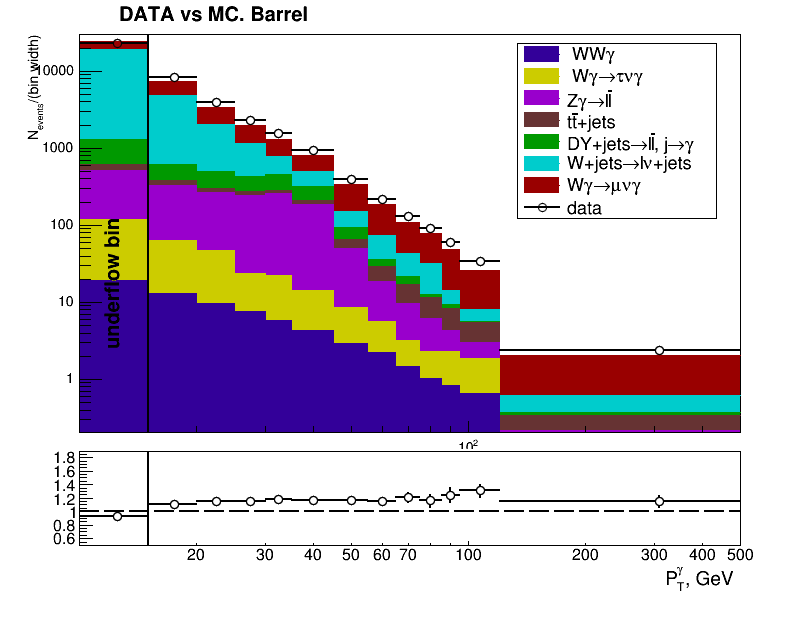
\includegraphics[width=0.48\textwidth]{../figs/figs_v11/MUON_WGamma/PrepareYields/c_TotalDATAvsMC_Barrel__phoEt.png}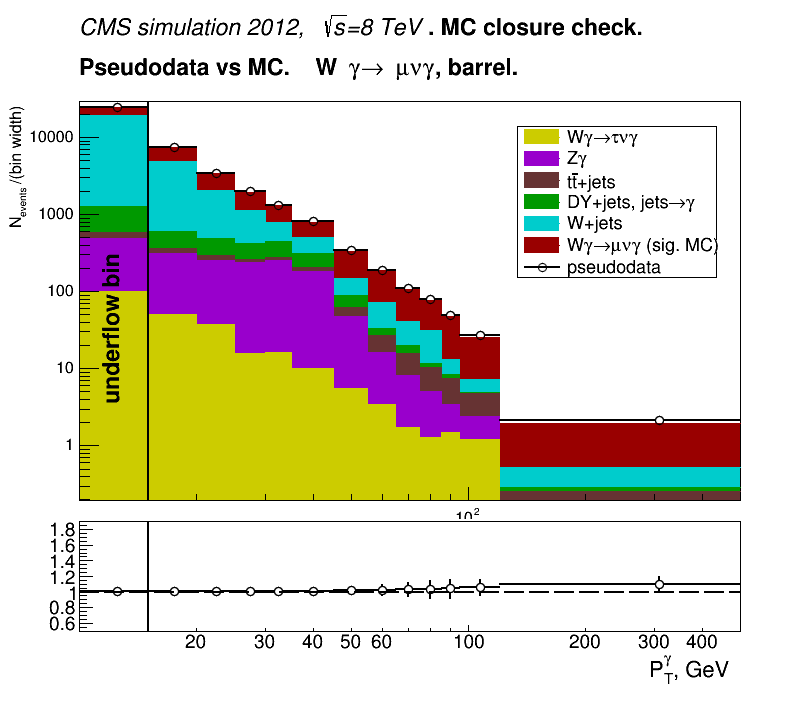
\includegraphics[width=0.48\textwidth]{../figs/figs_v11/MUON_WGamma/PrepareYields/c_TotalDATAvsMC_Barrel__phoEt_MCclosure.png}\\
   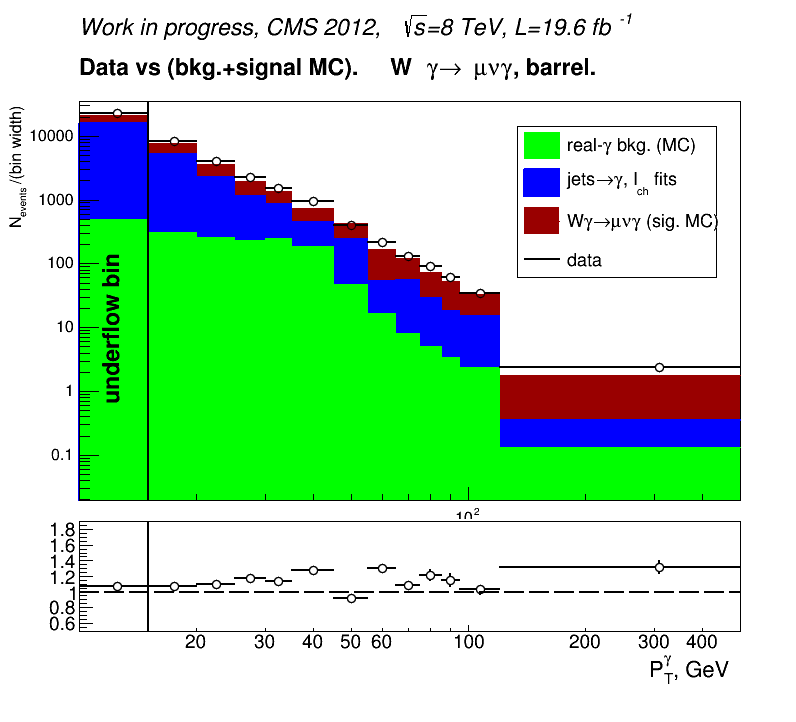
\includegraphics[width=0.48\textwidth]{../figs/figs_v11/MUON_WGamma/PrepareYields/c_DATAvsBkgPlusSigMCc_MUON_WGamma_TEMPL_CHISO_UNblind__Barrel__phoEt.png}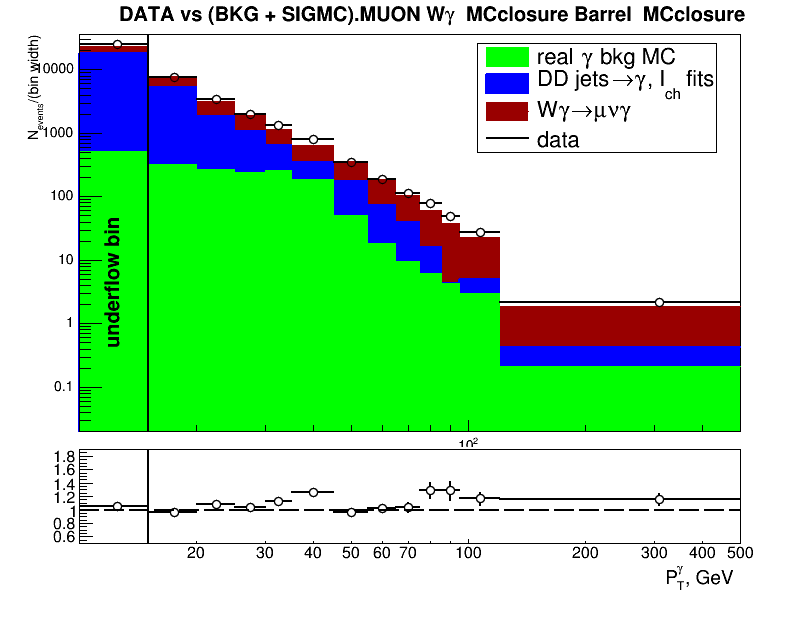
\includegraphics[width=0.48\textwidth]{../figs/figs_v11/MUON_WGamma/PrepareYields/c_DATAvsBkgPlusSigMCc_MUON_WGamma_TEMPL_CHISO_UNblind_MCclosure__Barrel__phoEt_MCclosure.png}\\
   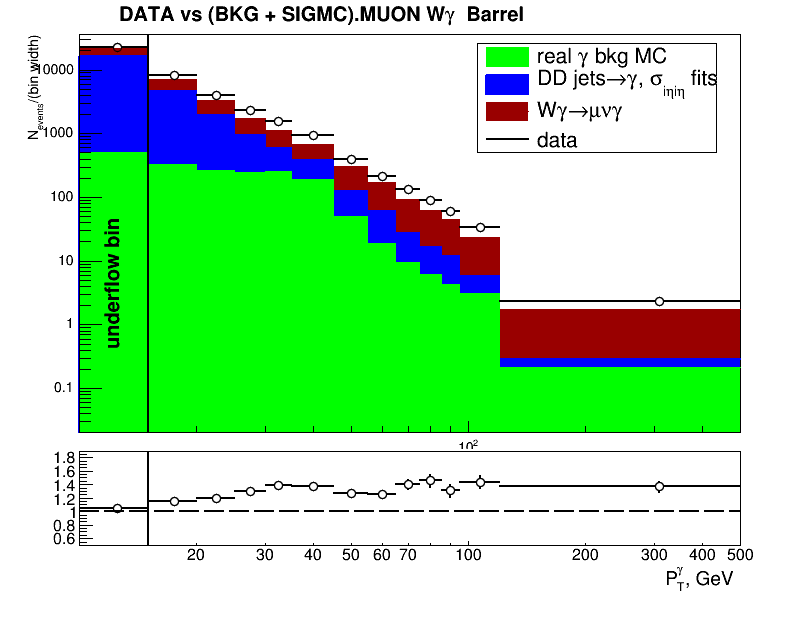
\includegraphics[width=0.48\textwidth]{../figs/figs_v11/MUON_WGamma/PrepareYields/c_DATAvsBkgPlusSigMCc_MUON_WGamma_TEMPL_SIHIH_UNblind__Barrel__phoEt.png}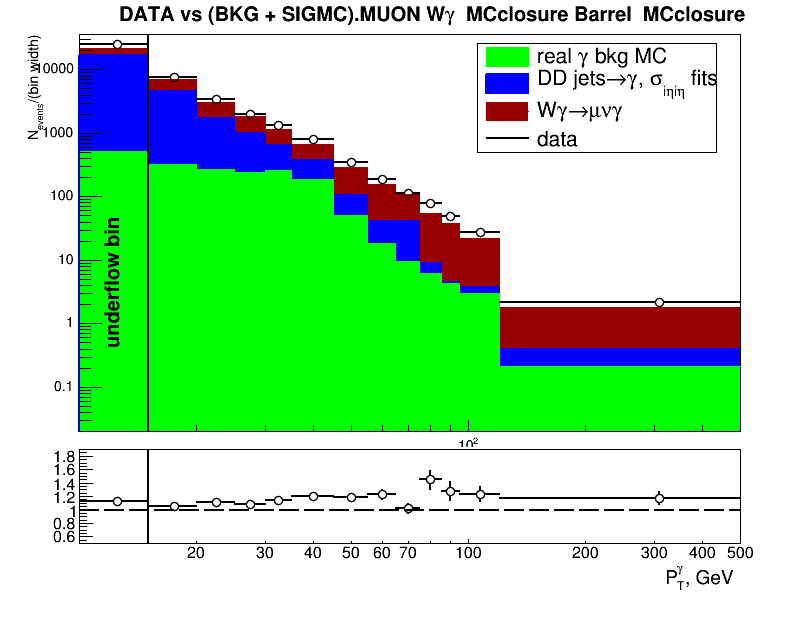
\includegraphics[width=0.48\textwidth]{../figs/figs_v11/MUON_WGamma/PrepareYields/c_DATAvsBkgPlusSigMCc_MUON_WGamma_TEMPL_SIHIH_UNblind_MCclosure__Barrel__phoEt_MCclosure.png}
  %\caption{Top: data (left) and pseudodata (right) vs MC. Middle and bottom: data (left) and pseudodata (right) vs background estimates and signal MC in bins of $P_T^{\gamma}$. Jets$\rightarrow\gamma$ background estimated from fits of $I_{ch}^{\gamma}$ (top) and  $\sigma_{i\eta i\eta}^{\gamma}$ (bottom). Muon channel. Barrel photons.}
  \caption{Data (left) and pseudodata (right) vs background estimates and signal MC in bins of $P_T^{\gamma}$. Jets$\rightarrow\gamma$ background estimated from fits of $I_{ch}^{\gamma}$ (top) and  $\sigma_{i\eta i\eta}^{\gamma}$ (bottom). Muon channel. Barrel photons.}
  \label{fig:DATAvsBKGandSIGMC_MCclosure_MUON_B}
  \end{center}
\end{figure}

\begin{figure}[htb]
  \begin{center}
%   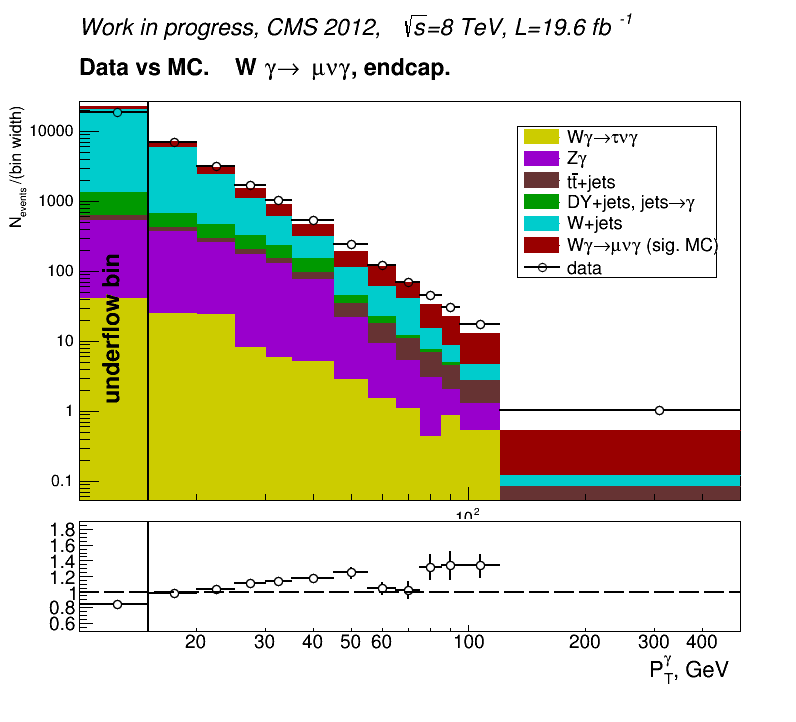
\includegraphics[width=0.48\textwidth]{../figs/figs_v11/MUON_WGamma/PrepareYields/c_TotalDATAvsMC_Endcap__phoEt.png}
%   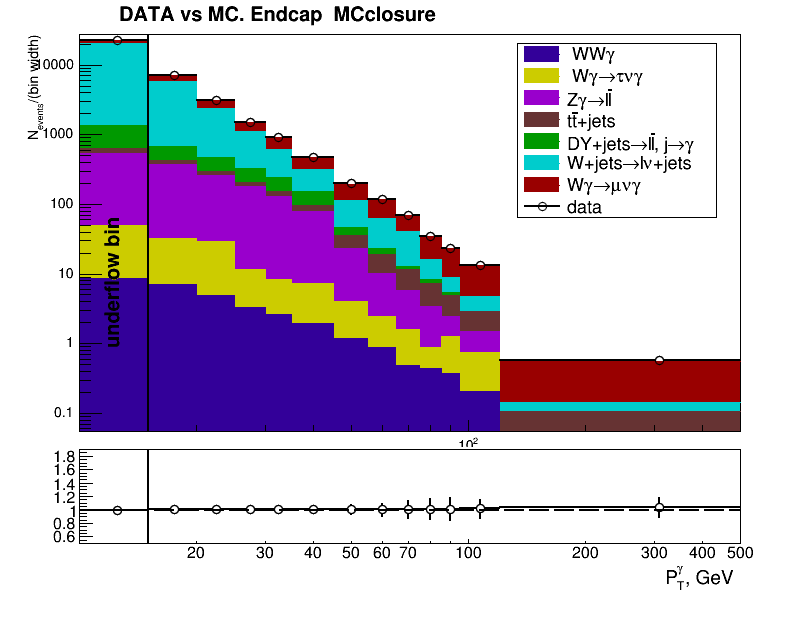
\includegraphics[width=0.48\textwidth]{../figs/figs_v11/MUON_WGamma/PrepareYields/c_TotalDATAvsMC_Endcap__phoEt_MCclosure.png}\\
   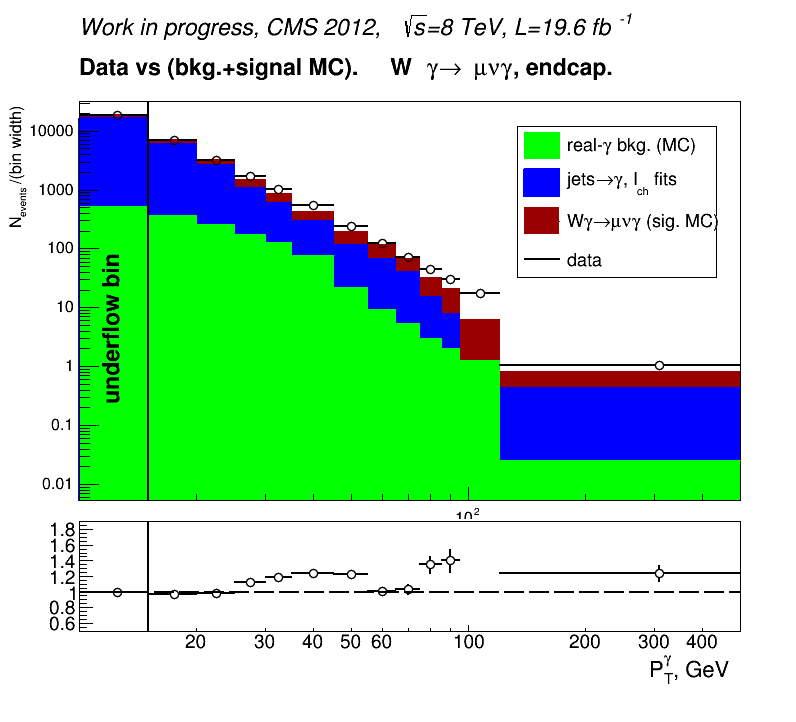
\includegraphics[width=0.48\textwidth]{../figs/figs_v11/MUON_WGamma/PrepareYields/c_DATAvsBkgPlusSigMCc_MUON_WGamma_TEMPL_CHISO_UNblind__Endcap__phoEt.png}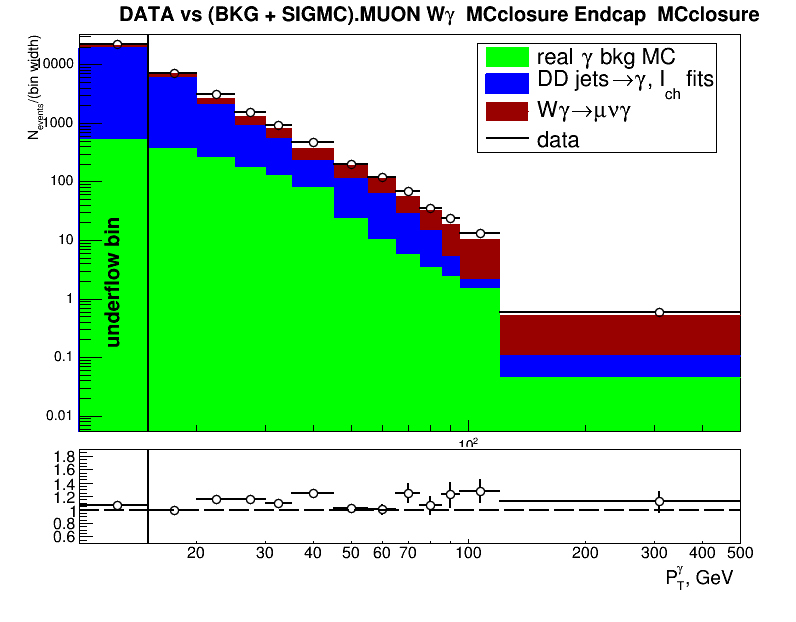
\includegraphics[width=0.48\textwidth]{../figs/figs_v11/MUON_WGamma/PrepareYields/c_DATAvsBkgPlusSigMCc_MUON_WGamma_TEMPL_CHISO_UNblind_MCclosure__Endcap__phoEt_MCclosure.png}\\
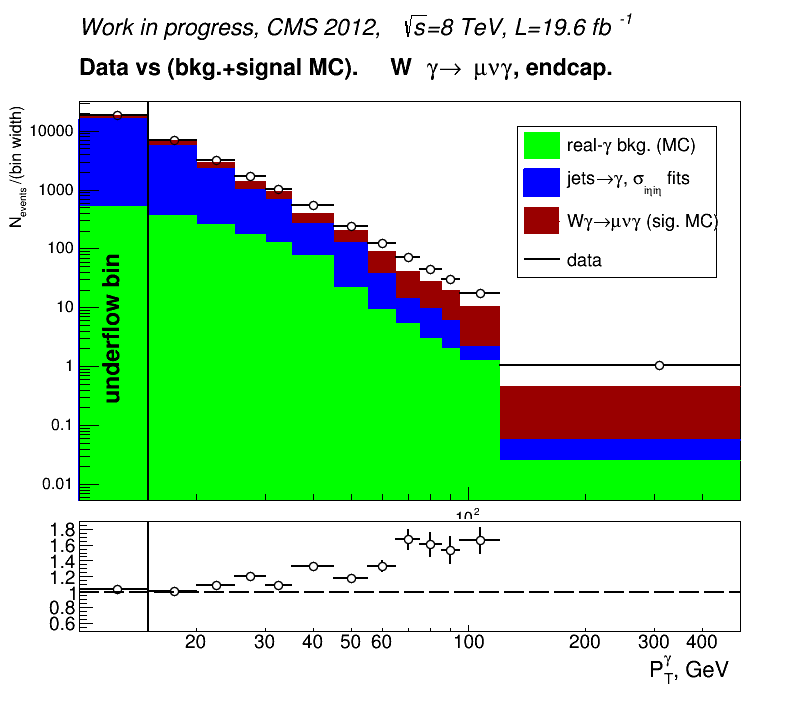
\includegraphics[width=0.48\textwidth]{../figs/figs_v11/MUON_WGamma/PrepareYields/c_DATAvsBkgPlusSigMCc_MUON_WGamma_TEMPL_SIHIH_UNblind__Endcap__phoEt.png}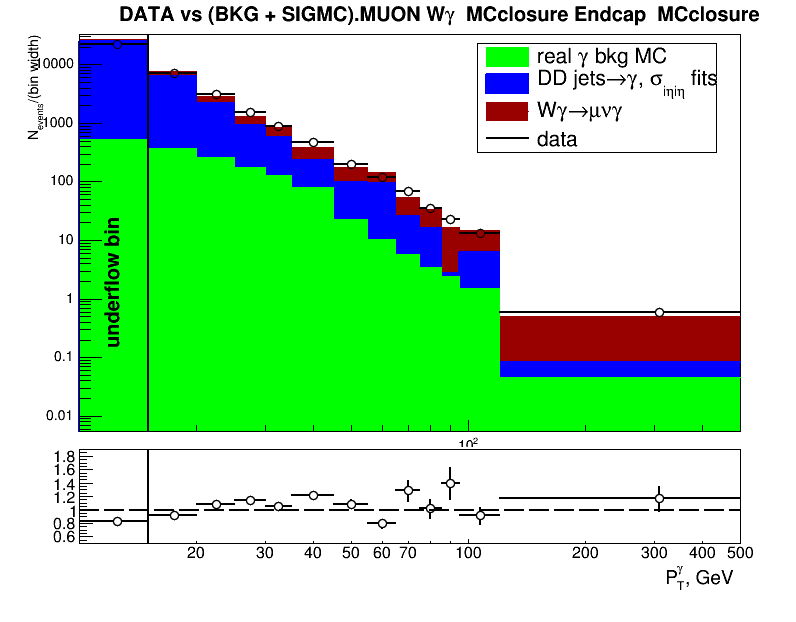
\includegraphics[width=0.48\textwidth]{../figs/figs_v11/MUON_WGamma/PrepareYields/c_DATAvsBkgPlusSigMCc_MUON_WGamma_TEMPL_SIHIH_UNblind_MCclosure__Endcap__phoEt_MCclosure.png}
  \caption{Data (left) and pseudodata (right) vs background estimates and signal MC in bins of $P_T^{\gamma}$. Jets$\rightarrow\gamma$ background estimated from fits of $I_{ch}^{\gamma}$ (middle) and  $\sigma_{i\eta i\eta}^{\gamma}$ (bottom). Muon channel. Endcap photons. }
  \label{fig:DATAvsBKGandSIGMC_MCclosure_MUON_E}
  \end{center}
\end{figure}

\begin{figure}[htb]
  \begin{center}
%   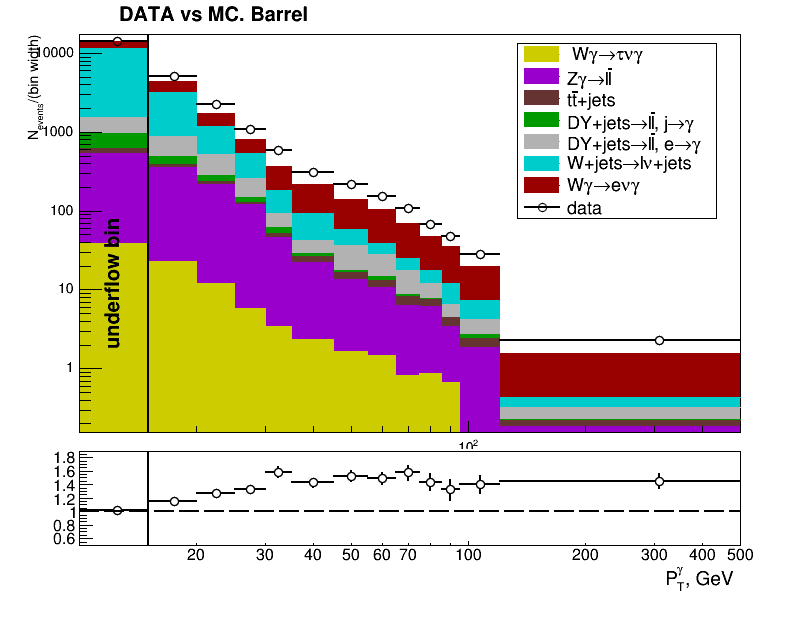
\includegraphics[width=0.48\textwidth]{../figs/figs_v11/ELECTRON_WGamma/PrepareYields/c_TotalDATAvsMC_Barrel__phoEt.png}
%   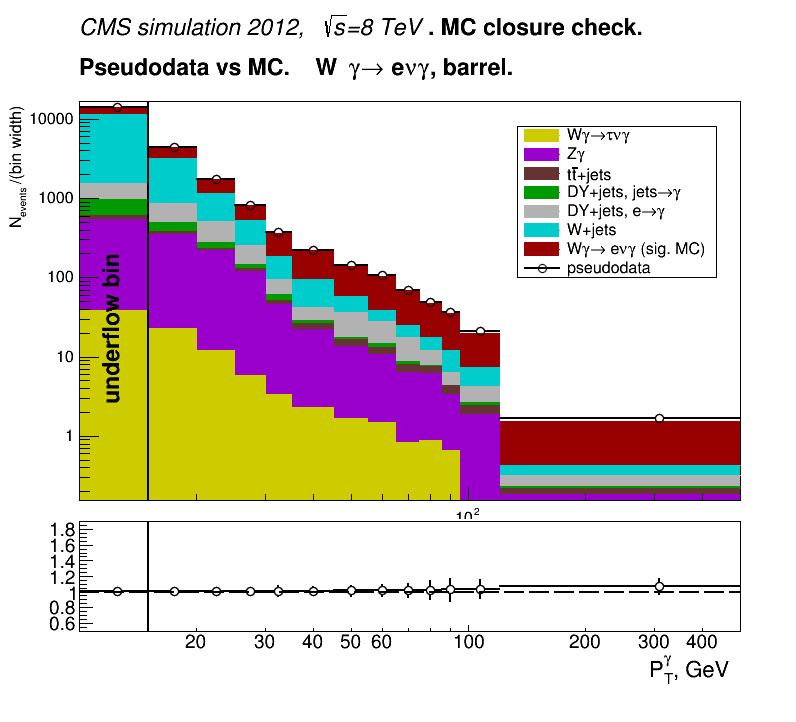
\includegraphics[width=0.48\textwidth]{../figs/figs_v11/ELECTRON_WGamma/PrepareYields/c_TotalDATAvsMC_Barrel__phoEt_MCclosure.png}\\
   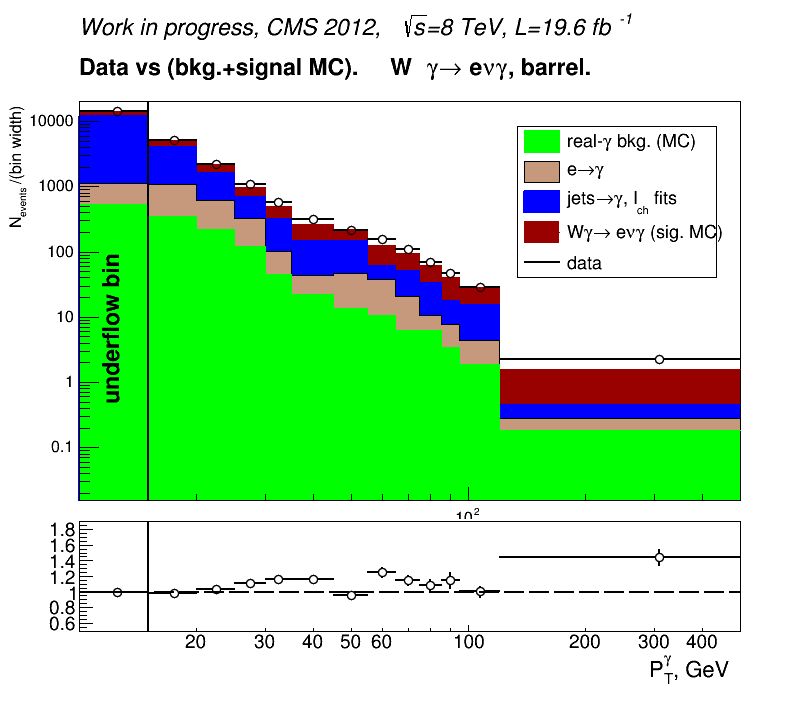
\includegraphics[width=0.48\textwidth]{../figs/figs_v11/ELECTRON_WGamma/PrepareYields/c_DATAvsBkgPlusSigMCc_ELECTRON_WGamma_TEMPL_CHISO_UNblind__Barrel__phoEt.png}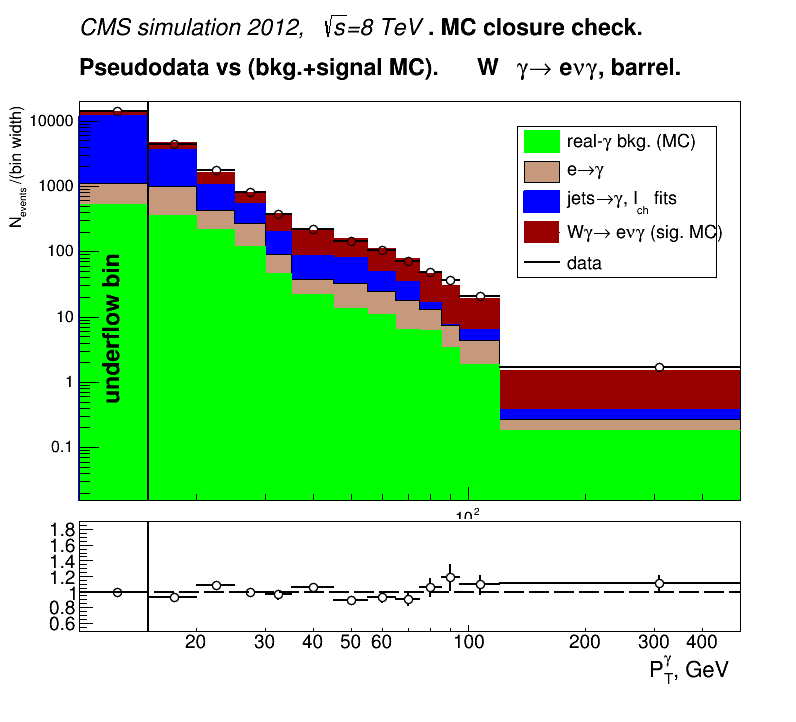
\includegraphics[width=0.48\textwidth]{../figs/figs_v11/ELECTRON_WGamma/PrepareYields/c_DATAvsBkgPlusSigMCc_ELECTRON_WGamma_TEMPL_CHISO_UNblind_MCclosure__Barrel__phoEt_MCclosure.png}\\
   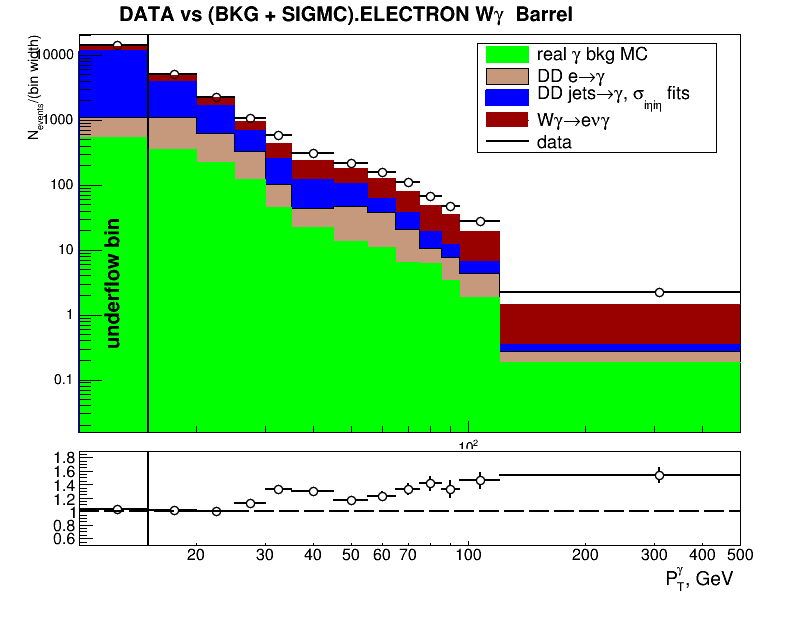
\includegraphics[width=0.48\textwidth]{../figs/figs_v11/ELECTRON_WGamma/PrepareYields/c_DATAvsBkgPlusSigMCc_ELECTRON_WGamma_TEMPL_SIHIH_UNblind__Barrel__phoEt.png}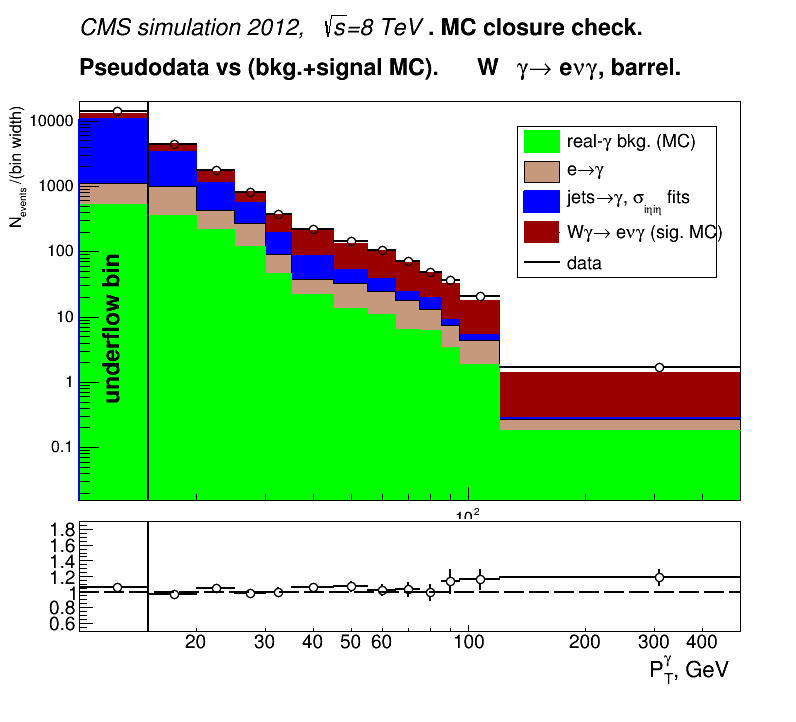
\includegraphics[width=0.48\textwidth]{../figs/figs_v11/ELECTRON_WGamma/PrepareYields/c_DATAvsBkgPlusSigMCc_ELECTRON_WGamma_TEMPL_SIHIH_UNblind_MCclosure__Barrel__phoEt_MCclosure.png}
  \caption{Data (left) and pseudodata (right) vs background estimates and signal MC in bins of $P_T^{\gamma}$. Jets$\rightarrow\gamma$ background estimated from fits of $I_{ch}^{\gamma}$ (middle) and  $\sigma_{i\eta i\eta}^{\gamma}$ (bottom). Electron channel. Barrel photons.}
  \label{fig:DATAvsBKGandSIGMC_MCclosure_ELECTRON_B}
  \end{center}
\end{figure}

\begin{figure}[htb]
  \begin{center}
%   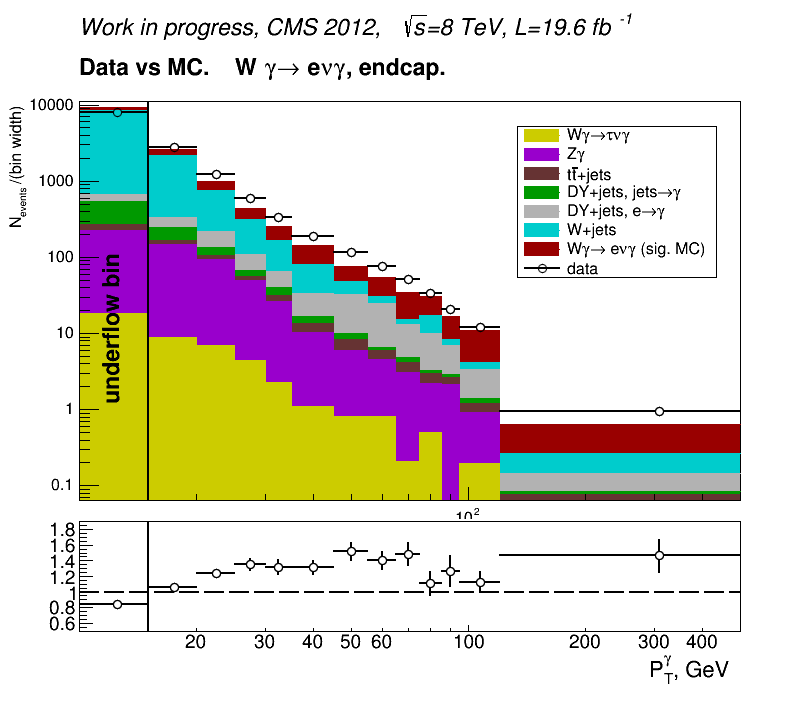
\includegraphics[width=0.48\textwidth]{../figs/figs_v11/ELECTRON_WGamma/PrepareYields/c_TotalDATAvsMC_Endcap__phoEt.png}
%   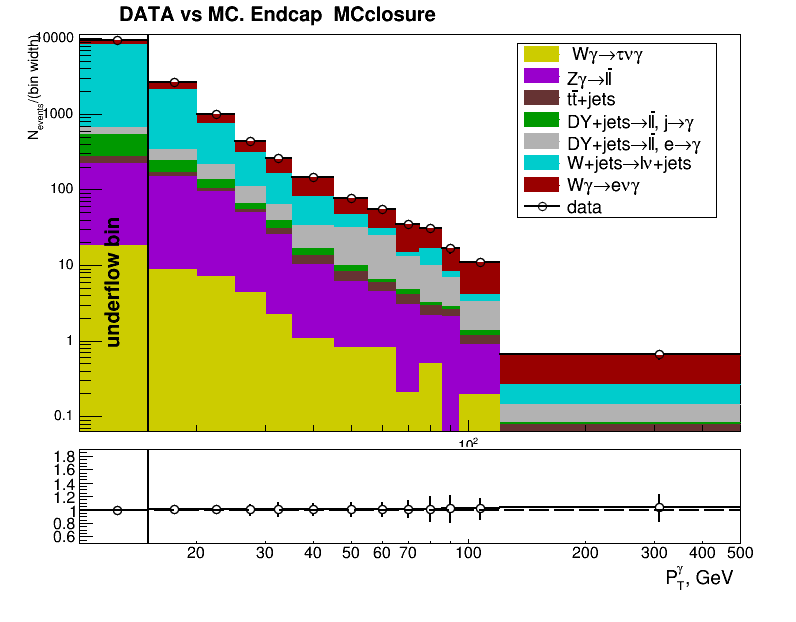
\includegraphics[width=0.48\textwidth]{../figs/figs_v11/ELECTRON_WGamma/PrepareYields/c_TotalDATAvsMC_Endcap__phoEt_MCclosure.png}\\
   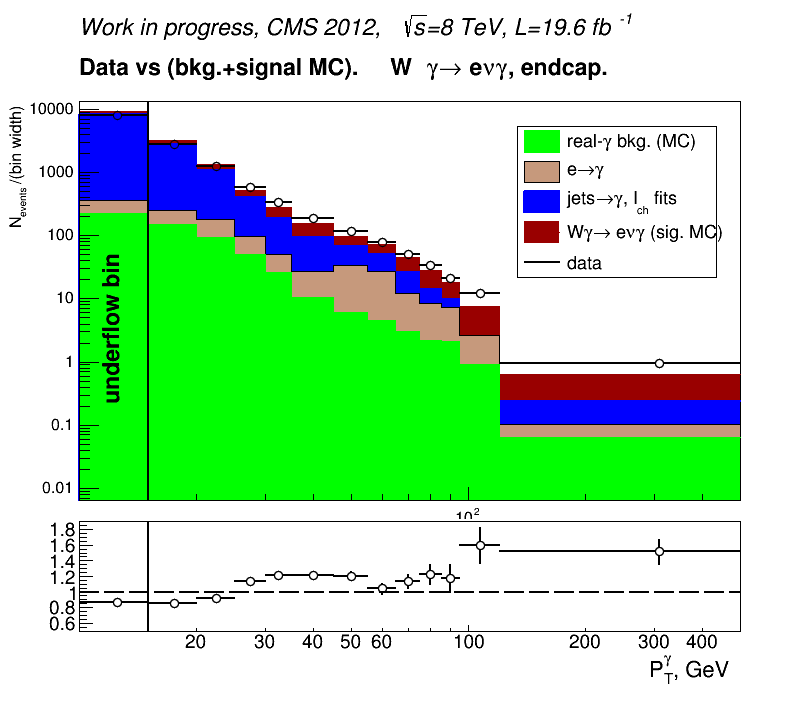
\includegraphics[width=0.48\textwidth]{../figs/figs_v11/ELECTRON_WGamma/PrepareYields/c_DATAvsBkgPlusSigMCc_ELECTRON_WGamma_TEMPL_CHISO_UNblind__Endcap__phoEt.png}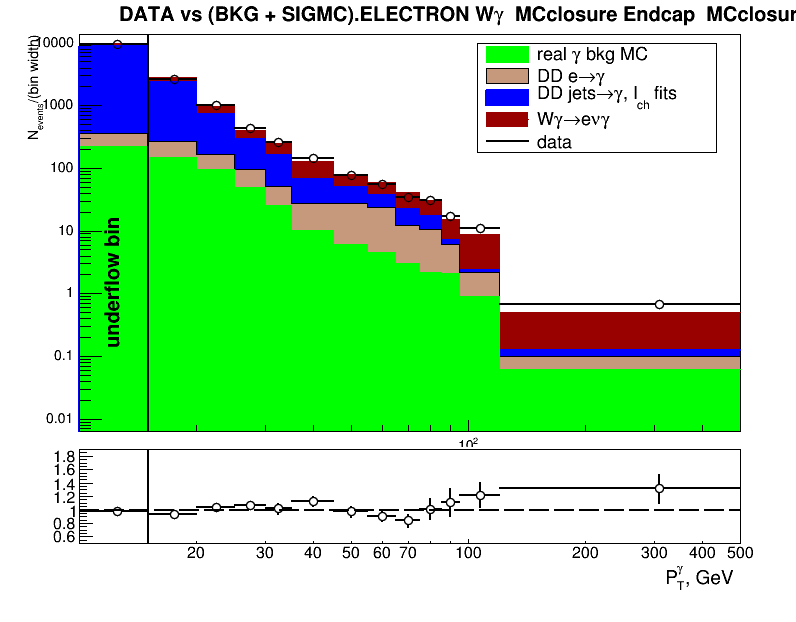
\includegraphics[width=0.48\textwidth]{../figs/figs_v11/ELECTRON_WGamma/PrepareYields/c_DATAvsBkgPlusSigMCc_ELECTRON_WGamma_TEMPL_CHISO_UNblind_MCclosure__Endcap__phoEt_MCclosure.png}\\
   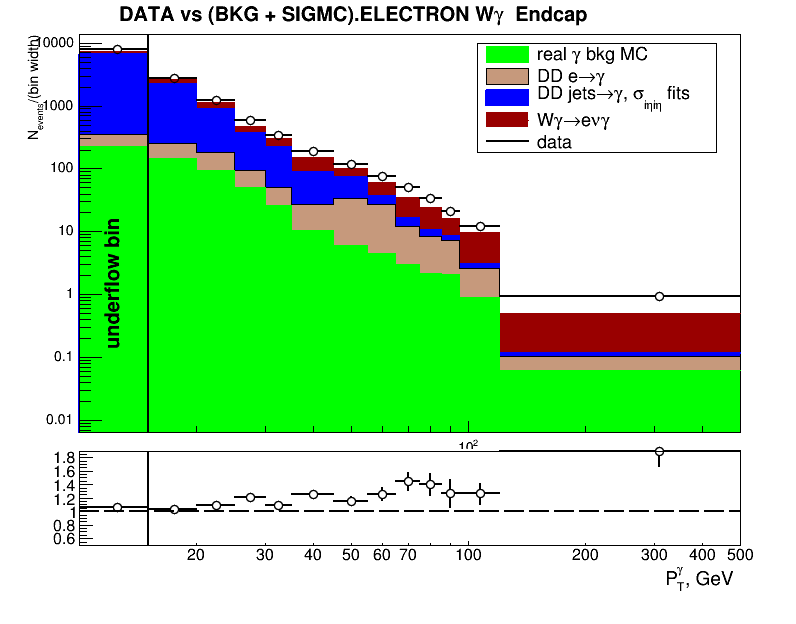
\includegraphics[width=0.48\textwidth]{../figs/figs_v11/ELECTRON_WGamma/PrepareYields/c_DATAvsBkgPlusSigMCc_ELECTRON_WGamma_TEMPL_SIHIH_UNblind__Endcap__phoEt.png}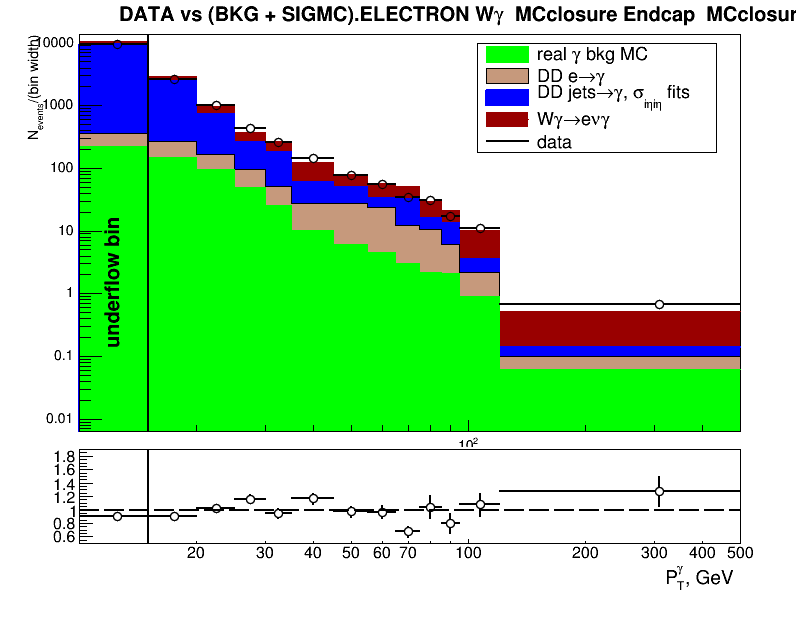
\includegraphics[width=0.48\textwidth]{../figs/figs_v11/ELECTRON_WGamma/PrepareYields/c_DATAvsBkgPlusSigMCc_ELECTRON_WGamma_TEMPL_SIHIH_UNblind_MCclosure__Endcap__phoEt_MCclosure.png}
  \caption{Data (left) and pseudodata (right) vs background estimates and signal MC in bins of $P_T^{\gamma}$. Jets$\rightarrow\gamma$ background estimated from fits of $I_{ch}^{\gamma}$ (middle) and  $\sigma_{i\eta i\eta}^{\gamma}$ (bottom). Electron channel. Endcap photons.}
  \label{fig:DATAvsBKGandSIGMC_MCclosure_ELECTRON_E}
  \end{center}
\end{figure}
